
%% bare_conf.tex
%% V1.3
%% 2007/01/11
%% by Michael Shell
%% See:
%% http://www.michaelshell.org/
%% for current contact information.
%%
%% This is a skeleton file demonstrating the use of IEEEtran.cls
%% (requires IEEEtran.cls version 1.7 or later) with an IEEE conference paper.
%%
%% Support sites:
%% http://www.michaelshell.org/tex/ieeetran/
%% http://www.ctan.org/tex-archive/macros/latex/contrib/IEEEtran/
%% and
%% http://www.ieee.org/

%\documentclass[conference]{IEEEtran}

%\usepackage{graphicx, color, code}
%\usepackage[cmex10]{amsmath}
%\usepackage{url}
% \usepackage{bookman}  %% bold teletype fonts, but don't know how to prevent it from changing the whole document

% Haven't figured out how to get this to work properly:
%\usepackage[\texttt{cmbtt}]{bold-extra}
% \usepackage{bold-extra} 

%\usepackage{courier}
%\usepackage{fancyvrb}

% correct bad hyphenation here
%\hyphenation{op-tical net-works semi-conduc-tor}


%====================================================================================================
%% FIRST, MISC USEFUL DEFINITIONS
%====================================================================================================

\definecolor{darkgreen}{rgb}{0, 0.5, 0}
\definecolor{darkblue}{rgb}{0,0,0.5}
\definecolor{mygrey}{rgb}{0.7,0.7,0.7}
\newcommand{\textblue}[1]{\textcolor{blue}{#1}}

\newcommand{\cde}[1]{{\footnotesize \tt #1}}

% \newcommand{\kw}[1]{{\bf{#1}}}
\newcommand{\kw}[1]{{\textbf{#1}}}

\newcommand{\comm}[1]{{\em \textcolor{darkgreen}{#1}}}  %% Code comments

\newcommand{\note}[1]{\begin{itemize}\item \textcolor{blue}{#1} \end{itemize}}

%% \newenvironment{mycode}
%% {% This is the begin code
%%   \begin{Verbatim}[commandchars=\\\{\}]}%
%%   %\footnotesize
%%   %\noindent
%%   %\begin{code}\noindent\vspace{-1mm}}
%% %  \begin{code}\noindent}
%% {% This is the end code
%%   \end{Verbatim}
%%   %\end{code} 
%% }

%% \newenvironment{inlinecode}
%% {
%%   \begin{center}
%%   \begin{minipage}{4in}
%%   \begin{mycode}
%% } 
%% {
%%   \end{mycode}
%%   \end{minipage}
%%   \end{center}
%%   \vspace{-1.5ex}
%% }

%% ============================================================
%% USE TO DISABLE COMMENTS:
 \def\noeditingmarks{}
%% ============================================================
\ifx\noeditingmarks\undefined
   \newcommand{\textred}[1]{\textcolor{red}{#1}}
   \newcommand{\pgwrapper}[2]{\textred{#1: #2}}
%   \newcommand{\pgwrapper}[2]{}
   \newcommand{\rnote}[1]{\begin{itemize}\item{\textcolor{blue}{#1}}\end{itemize}}
   \newcommand{\new}[1]{\textcolor{blue}{#1}}
   \newcommand{\const}[1]{\textred{#1}}

%% RRN: Dim the background for Ryan's eyes:
%%   What I need here is a way to do it based on user or host name...
% \pagecolor{mygrey}

\else
   \newcommand{\textred}[1]{#1}
   \newcommand{\pgwrapper}[2]{}
   \newcommand{\rnote}[1]{}
   \newcommand{\new}[1]{#1}
   \newcommand{\const}[1]{#1}
\fi

\newcommand{\js}[1]{\pgwrapper{BJS}{#1}}
\newcommand{\rn}[1]{\pgwrapper{RRN}{#1}}


%% Can we call our ``things'' 
%% ArBB/Haskell for the bindings part ? 
%% Accelerate/ArBB for the Accelerate backend ?
%% This would work with the convention we adopted for 
%%      ArBB/C++  
\newcommand{\systemname}[0]{{Harbb}}
%\newcommand{\systemname}[0]{\textred{HArBB}}

%% This could in theory be separate from the project name..
\newcommand{\accarbb}[0]{\systemname{}}

%% NOTE: THIS SHOULD BE THE SAME AS SYSTEMNAME:
\newcommand{\arbbvmH}[0]{ArBB/Haskell}


%====================================================================================================
% END DEFINITIONS
%====================================================================================================




%\begin{document}
% \title{Painless Portable Vector Parallelism\\ with Haskell and Intel ArBB}
%\title{Programming Future Parallel Architectures\\ with Haskell and Intel ArBB}
% \title{Embedded Domain-Specific Languages Pave the Way for New Parallel Architectures}

%\author{\IEEEauthorblockN{Bo Joel Svensson}
%\IEEEauthorblockA{Dept. of Computer Science and Engineering\\
%Chalmers University of Technology\\
%Gothenburg, Sweden\\
%Email: joels@chalmers.se}
%\and
%\IEEEauthorblockN{Ryan Newton}
%\IEEEauthorblockA{Intel Corporation\\
%Hudson, MA\\
%Email: rrnewton@gmail.com
%}}
% Email: ryan.r.newton@intel.com

%\maketitle

%\begin{abstract}
%
\subsection*{Abstract}
New parallel architectures, such 
\new{as Cell, Intel MIC, GPUs, and tiled architectures, enable} high
performance but are often hard to program.
What is needed is a bridge between high-level programming models 
where programmers are most productive and modern parallel architectures. 
We propose that that bridge is Embedded Domain Specific Languages (EDSLs). 

\new{One attractive target for EDSLs is}
Intel ArBB, a virtual machine for parallel, vectorized computations.
% that serves as a compilation target for EDSLs.
We propose to wed ArBB with the functional programming language
Haskell, {using an EDSL} that generates code for the ArBB VM.  This Haskell integration provides 
% a determinism guarantee 
added safety guarantees compared to other ArBB interfaces.
%
Further, our prototype, \systemname{}, is one of the first EDSL implementations with
optimized backends for multiple parallel architectures (CPU, \new{NVIDIA GPU}, and
others), allowing portability of source code over devices
and their accelerators.


%\end{abstract}
%\IEEEpeerreviewmaketitle




% ====================================================================================================
\subsection{Introduction}
% ====================================================================================================

Are radical new parallel architectures market-feasible if they require
significant changes for programmers?  The jury is out.  In recent
years we have seen difficult-to-program chips suffer 
% \cite{cell} 
(e.g. Cell)
and
GPU vendors strive to enable more traditional programming features
\cite{fermi} (e.g. C++).  There is an increasing
tension between ease of programming and efficiency.

The tension  shows  across diverse chip markets.  For example,
small embedded devices are most power efficient if their processors and operating systems
omit programming features such as virtual memory and threads \cite{tinyos}.  
At the other end of the power spectrum, GPU's
graphics performance may suffer due to inclusion of hardware to ease
GPGPU programming.  In short, there is an opportunity cost to
including extra hardware for programmability.

In this paper, we argue 
that a specific technique holds the greatest promise of solving the programmability dilemma.
%
Domain-specific languages, {\em embedded} within general purpose
languages (EDSLs) 
 enable familiar programming models 
{\em and} flexible
mapping onto new hardware.  The key to having this cake and eating it
too is {\em metaprogramming}.  Familiar programming features are
present, but are eliminated at an intermediate (metaprogram evaluation)
phase and therefore do not reach the parallel hardware itself.


% We present our ongoing work on a
In pursuit of this vision, we offer a
% 
 new EDSL implementation, called \accarbb{}, that combines
existing systems, Accelerate \cite{ACCELERATEDAMP11} and ArBB \cite{ArBB}, to produce a unified
high-level programming environment equally suited to multicore,
vectorized CPUs, as to GPUs and other accelerators (such as Intel MIC chips \cite{larrabee}).
%
\if{0}
ArBB is based on the RapidMind \cite{RapidMind} system which was an embedded 
DSL targeting multicore CPUs as well as GPUs. ArBB does not \new{yet} include a GPU 
backend like RapidMind, targeting multicore CPUs and their vector 
units. 
\fi{}
\systemname{} is a single EDSL implementation 
with independently optimized backends \new{by different teams; 
namely, the ArBB backend for CPU/MIC, and a CUDA backend for NVIDIA GPU.}
This makes
\systemname{} an appealing platform for fair CPU/GPU comparisons, 
as well as a compelling programming model for single-source portable performance across a range of
parallel architectures, \new{present and future}.
%%To our knowledge, \systemname{} is the first EDSL implementation with
%%independently optimized backends for CPUs and GPUs.  This makes
%%\systemname{} an appealing platform for fair CPU/GPU comparisons, 
%%as well as a compelling programming
%%model for single-source portable performance across a range of
%%parallel architectures.


% ====================================================================================================
\subsection{Embedded Domain-Specific Languages}
% ====================================================================================================


Domain-specific languages---from Makefiles and \LaTeX{} to
Matlab---are almost too ubiquitous to notice.  Most relevant to our
purposes, domain-specific languages (DSLs) that target a narrow domain and expose communication
patterns to the compiler 
 have achieved performance-portability across a wide range of parallel
architectures.  
StreamIt\cite{streamit} is a good example.
% (for example, StreamIt\cite{streamit})
% The high-water mark in this area is perhaps  StreamIt\cite{streamit}.
% 

% It has been noted \cite{not-sure} that 
% Yet the few DSLs that gain popularity lose simplicity\cite{not-sure}.  
% Yet popular DSLs rarely remain simple \cite{not-sure}.  
DSLs may start out simple and focused, but if they gain popularity
they quickly grow in complexity to rival full-blown languages.
Feature creep
can make DSL implementations complex and expensive to maintain.
Further, non-standard DSL syntax and features present a learning curve for users.  In the
last ten years an attractive solution to this dilemma has emerged: {\em
  embed} each DSL into a general-purpose host language that can provide
common functionality with familiar syntax and semantics.
% in place of the DSL.

When embedding, host language programs {generate} DSL programs;
% Embedding means that the host language is used to generate DSL programs; 
the {\em deeper} the embedding, the more integrated the
DSL into the syntax and type-system of the host language.
%
% Typically, %% pruning weasel words
A key host-language feature for embedding is that
language constructs can be overloaded to operate over {\em abstract
  syntax trees} (ASTs)\footnote{This ad-hoc polymorphism is accomplished,
for example, through operator-overloading in C++ or type classes in
Haskell.}.  For example, the following simple function operates on scalars:


\vspace{1mm}
\begin{Verbatim}[commandchars=\\\{\}]
  float f(float x) \{ return (2*x - 1); \}
\end{Verbatim}
\noindent
But simply by changing the types, \cde{f} might be lifted to operate on {\em
  expressions} (which, when evaluated, will yield \cde{floats}):

\vspace{1mm}
\begin{Verbatim}[commandchars=\\\{\}]
  \kw{exp<float>} f(\kw{exp<float>} x) \{
    return (2*x - 1);
  \}
\end{Verbatim}

A common arrangement is for the host language program to execute at
runtime but to generate ASTs that are executed by a just-in-time
(DSL) compiler.  This use of metaprogramming (program generation)
differs from the more common usage of preprocessors and 
% Lisp/Scheme macros \cite{scheme-macros}
macros, which typically add extra
phases of computation {\em before}  compile time---increasing
the number of compile-time rather than runtime phases.

% EDSLs typically add additional runtime phases.  That is, the host language program 
% executes at runtime but uses a JIT to process generated ASTs.
%% which are
%% usually used to perform computation {\em earlier} than the usual
%% compile time, embedded DSLs (EDSLs) typically defer computation 


One reason that EDSLs are good for productivity is that the programmer
gains the software engineering benefits of the host language
(object-orientation, higher-order-functions, modules, etc), while not
paying the cost at runtime for additional layers of abstraction or
indirection.  Indeed, the embedded languages for 
performance-oriented EDSLs are often simple, first-order
languages without pointers \cite{wavescript, ACCELERATEDAMP11}.

% , paul-lius-thingy

% regiment,
As a research area, EDSLs and two-stage DSLs have been actively pursued for at least a
decade \cite{VERTIGO, wavescript} but are gaining steam
recently 
%\cite{sejits, stanford-ppl} 
\cite{copperhead, stanford-ppl} 
and are beginning to appear in
commercial products \cite{ArBB}.
%
Further, EDSL techniques have spread beyond their origin in 
 the programming languages community.
% 
For example, both Stanford's Parallel Programming Laboratory (PPL) and
the Berkeley Parlab are creating EDSLs as their flagship parallel
programming solutions for domains such as machine learning and
rendering \cite{stanford-ppl}.
  Moreover, EDSLs need not be hosted by esoteric research languages---Intel's
 ArBB embeds an array language in C++ and Berkeley's
Copperhead \cite{copperhead} generates CUDA from simple Python code.

%\rnote{Is there a good motivating example program?  What are some of
%  the Metaocaml motivating examples?}

{For the remainder of this paper we will focus our discussion
  on the Intel ArBB VM, a virtual machine for just-in-time
  generation of vector codes, \new{which implements a restricted} domain-specific
  language of array computations.  In this paper we introduce
  {\em High-level ArBB}, 
  (\systemname{}), an EDSL that internally uses the ArBB
  VM.  \new{While Intel's ArBB package already includes an EDSL targeting the VM (for C++)},
\systemname{} \new{offers additional advantages, including}
  more succinct programs and additionally safety
  guarantees---namely, complete deterministic-by-construction parallel
  programs (across both host and VM languages).}


% ====================================================================================================
% \section{Accelerate and ArBB}
%\section{\accarbb{}:  ArBB and Accelerate}
\subsection{\accarbb{} $=$ ArBB $+$ Accelerate}
\label{sec:accelerate-arbb}
% ====================================================================================================

Our first \systemname{} prototype adapts an existing EDSL called {\em
  Accelerate} (Data.Array.Accelerate).  Accelerate targets high-level
data-parallel programming in Haskell.
Previous work on Accelerate has focused on developing a CUDA-backend
for GPU programming.  In this paper we describe our effort to retarget
Accelerate to ArBB.  

With respect to determinism guarantees, the existing Intel ArBB product
represents an integration of the safe (ArBB VM) with the unsafe (C++).
In the Haskell context, because purely functional computations are
guaranteed deterministic (even when executed in parallel), and because
ArBB computations invoked by Haskell functions are themselves free of
side-effects, \systemname{} achieves a
guarantee of determinism for complete programs that combine both
Haskell computation and ArBB VM computation.
% which offers portability.
% (The 'H' in \systemname{} therefore stands for Haskell as well as ``High-level''.)


%% {\em Accelerate} (Data.Array.Accelerate) is an existing EDSL for 
%% high-level data-parallel programming in Haskell~\cite{Accelerate}. 
The Accelerate programming model consists of collective 
operations that can be performed over arrays, together with a simple 
language of scalar expressions\new{---in the current release, the Haskell type system enforces that parallelism not be nested.}
\if{0}
The Haskell type 
system is used to enforce that no nested data-parallelism can be expressed 
\new{(in the current release, this may be relaxed in the future).}
\fi{}
Accelerate's collective operations include {\em Map} (akin to parallel
for loops) {\em ZipWith} (a generalization of elementwise vector addition) and 
{\em Fold} (sum generalized)---familiar operations for programmers versed in the functional paradigm.
All of these collective operations are easily parallelizable. 
% In the case of {\em Map} and {\em ZipWith} the potential for parallelism is abundant.  

%% dotProd :: Vector Float -> 
%%            Vector Float -> 
%%            Acc (Scalar Float) 
\begin{Verbatim}[commandchars=\\\{\}]
dotProd (xs :: Vector Float) 
        (ys :: Vector Float) = 
  \kw{let} xs\_ = use xs 
      ys\_ = use ys 
  \kw{in}  fold (+) 0 (zipWith (*) xs\_ ys\_) 
\end{Verbatim}

The Accelerate code listing above specifies a function that takes two 1-dimensional 
arrays as inputs (of type \cde{Vector Float}, e.g. a vector of floats). The result of the function is a single
scalar. 
% (\cde{Scalar Float})
The \cde{use} function is applied to an array to convert it 
for use in the collective operations provided by Accelerate;
\cde{use} 
% is actually a function with type \cde{Vector a -> Acc (Vector a)} and 
may result in
copying the array to, for example, the GPU in the case of Accelerate's 
CUDA backend.  

After applying \cde{use} to bring in input data, the programmer then
constructs a data-parallel program from collective operations.
Above, \cde{fold} is a function that takes three arguments, 
here those arguments are \cde{(+)},  $0$ and \cde{zipWith (*) xs\_ ys\_}. 
\cde{zipWith}, in turn, is a function taking three arguments, \cde{(*)}, 
\cde{xs\_} and \cde{ys\_}. The \cde{zipWith} operation here applies pairwise 
multiplication to the two arrays and the \cde{fold} sums up all the elements 
into a single scalar. 

%\rn{Following para slightly redundant but ok...}
%Accelerate makes GPU programming accessible to the functional programmer 
%by offering a familiar set of operations. This set of operations also have 
%the beneficial property that they have inherent parallelism and are 
%easily implementable on the GPU. 

Accelerate's CUDA backend implements collective operations using
a hand-tuned ``skeleton'' for each operation (and possibly for
different hardware versions). The kernel---for example, the function
to mapped over the dataset---is 
instantiated into the body of the skeleton code. The resulting 
program is compiled using the NVIDIA CUDA compiler and dynamically linked 
into the running Haskell program.

%\subsection{Intel Array Building Blocks (ArBB)}
\subsection{Intel Array Building Blocks (ArBB)}
\label{sec:arbb}

%ArBB is embedded in the C++ programming language but it also exposes a 
%very low level API that is purely C. 
%{\em ArBB} (Array Building Blocks) is also an embedded DSL. 
The operations exposed by ArBB are similar to those of Accelerate. 
In ArBB, parallel computations are expressed using a set of built-in 
primitives. All vectorization and threading is managed internally by 
ArBB. The programmer uses collective operations with a clear semantics 
such as \cde {add\_reduce} that computes the sum of the elements in a given 
array. ArBB also has language constructions for control flow, conditionals
and loops. These operations have their usual sequential semantics and are not 
parallelized by the system, rather, only specific collective operations are executed
in parallel. 

Today's existing ArBB product is embedded in C++ and provides special
types for scalars and arrays (e.g. \cde{dense<f32>} rather than \cde{vector<float>}).
Using ArBB/C++ to express the dot product computation can be done 
as follows:

%\vspace{2mm}
\begin{Verbatim}[commandchars=\\\{\}]
\kw{void} dot\_product(\kw{const} dense<f32>& a, 
                 \kw{const} dense<f32>& b,
                 f32& c) 
{ 
  c = add\_reduce(a * b);
}
\end{Verbatim} 


% The above program takes two arrays of type \cde{dense<f32>} as input. 
% \cde{dense<f32>} specifies a 1-dimensional array of 32-bit floating
% point values. The result is a single 32-bit float.  

Note that arithmetic operators such as (*) are overloaded 
for to operate on arrays as well as scalars (e.g. \cde{a * b} above).
Thus, the above C++ function multiplies two arrays before summing them with \cde {add\_reduce}:

The code listing below is indicative to the amount of glue code needed to invoke an 
ArBB computation\footnote{In OpenCL and CUDA the glue code situation is even worse}. It shows how the dot product code is launched using {\tt call} and 
how data is bound, {\tt bind}, for use in ArBB. 

\vspace{2mm}
\begin{Verbatim}[commandchars=\\\{\}]
\kw{int} main() 
{ 
  double a[SIZE];
  double b[SIZE];

  for ( \kw{int} i = 0; i < SIZE; ++i) { 
    a[i] = ...; b[i] = ...;
  }
  dense<f32> va, vb;
  f32 vc;
  bind(va, a, SIZE); 
  bind(vb, b, SIZE); 
  call(dot\_product)(va, vb, &vc); 
  ...
}
\end{Verbatim}


%\rnote{SPECIFICALLY ADDRESS THE FUNCTIONALITY GAP?  E.G general
%  reduce.  Any other examples?}

The model provided by Accelerate is slightly richer than that of ArBB.
Even the two very simple \cde {dot\_product} examples above manage to illustrate 
this. In Accelerate there is a more general reduction primitive called \cde {fold} 
where in ArBB there are specific reductions, \cde {add\_reduce}, \cde {mul\_reduce} 
and so on. Not visible in these small examples is another difference, Accelerate 
operations are generalized to arbitrary dimensions while ArBB operations are 
limited to 1, 2, and 3 dimensions (and 0, i.e. scalar). These differences aside,
the ArBB and Accelerate programming models are very similar.


% ====================================================================================================
\subsection{Implementation of \systemname{}} 
% ====================================================================================================


%\rnote{Sadly the Haskell details don't buy us much here... what are
%  the {\em conceptual} problems solved in mapping the Accelerate
%  abstraction to the ArBB one?  The data models are similar, but
%  there are always mismatches -- dimensionality support, missing
%  reduction.}

%\rnote{What is the technique that you are using to address these sorts
%  of problems?  Is there anything to say about it?}

\begin{figure}
  \begin{center}
   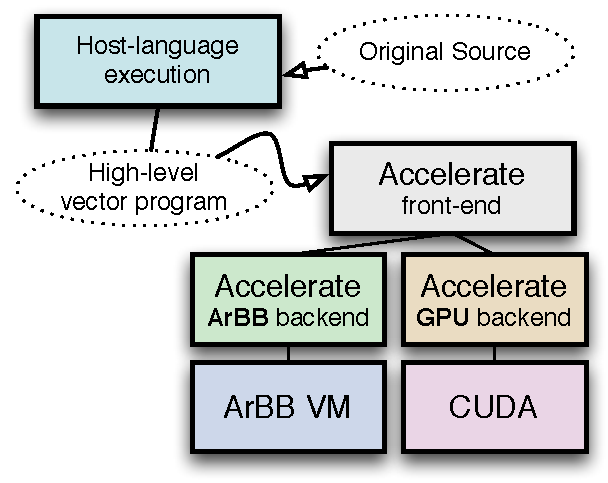
\includegraphics[width=2.0in]{./arbb/figure_architecture}    
  \end{center}
\vspace{-5mm}
  \caption{Architecture of the \systemname{} system.  \rn{(ROUGH.)}}
  \label{f:architecture}
\end{figure}


Using Accelerate and ArBB together, we propose a layered architecture
for \systemname{},
% Our goal is to make the benefits of ArBB available to the Haskell programmer. 
% \js{(Or is our goal to give an even better ``front-end'' to ArBB compared to C++)}
% We propose that this is best accomplished using a layered approach, as
pictured in Figure~\ref{f:architecture}. 
The host language execution (via Haskell in this case) executes the
programmer's source code, generating a vector program in the
restricted language of the Accelerate front-end.
Then either Accelerate backend---ArBB or CUDA---may be used.
The 
bottom layer of the ArBB backend consists of a direct mapping of the ArBB virtual machine
API (VMAPI) into Haskell including one-to-one bindings for each C 
function. 
To [partially] automate the creation of these bindings we used the C2HS system \cite{C2HS}. The 
\arbbvmH{} bindings are very low-level.
%and make little use of the high-level programming methods that
% Haskell programmers want. 
The idea 
is that the \arbbvmH{} bindings should be used to implement
backends for higher-level data-parallel EDSLs.

%% To illustrate our position we 
%% have started working on a backend to the successful DSL Accelerate 
%% (Data.Array.Accelerate) using our \arbbvmH{} bindings. 

To address the functionality mismatch between Accelerate and ArBB,
when possible we reencode the users Accelerate program using existing
ArBB mechanisms.  Our prototype does not support 100\% of Accelerate's
compute model (for example, only supporting  up to three-dimensional
arrays), but the remaining functionality can be mapped onto ArBB in
time using known methods---for example, our compiler could map higher
dimensional arrays onto a specific lower-dimensional data-layout.

%% The programming models supported by ArBB and Accelerate are very similar. 
%% Both obtain their parallelism by exposing collective operations 
%% such as {\em Map}, {\em Reduce}, {\em ZipWith} and {\em Scan} (all prefixes operations). However, 
%% the functionality match is not 100\%. For example, Accelerate supports {\em Map} operations 
%% over N-dimensional Arrays while ArBB supports them only up to 3-dimensions. 
%% Similar inconsistencies apply to the other operations as well. \textred{The current
%% ArBB backend simply disallows Accelerate programs using too high dimensionality
%% of the arrays.} \rn{Sure, we want to say that we're not done closing
%%   this gap (for
%%   accuracy) but more importantly we want to identify whether
%%   techniques exist to close the gap.  Presumably, yes?  We can
%%   ourselves collapse the dimensionality of arrays before giving them
%%   to ArBB?  Are there any operations that would defeat that technique?}
%

One example of a functionality discrepancy bridged by our
implementation is reductions.  As mentioned in \ref{sec:arbb},
Accelerate allows the programmer to reduce using an arbitrary
associative function, but ArBB has only built-in reductions with fixed
operations (add, multiply, xor, etc). We plan to provide general reductions in
the ArBB backend by a two-fold strategy:

\begin{enumerate}
\item Attempt to map an Accelerate reduction directly onto an ArBB
  primitive such as \cde{add\_reduce}.
\item Apply a general reduction technique based on $log(N)$ map
  operations over successively halving array sizes.  Essentially, cut
  the array in half, combine the halves, repeat. In ~\cite{reduction}
  this approach is explained in the context of CUDA. 
\end{enumerate}

%% \rn{Is the technique worthy of
%%   description?  Can we just cite the CUDA documentation or something
%%   since it's common?} 

In our current experiments, approach (2) is significantly slower.
Therefore, the ideal would be that ArBB exposed general reduction
directly in its programming model.  We expect this functionality to be
added in future releases.  In the meantime we plan to explore a
technique that would allow us to maximize the number of situations in
which (1) above applies.  Namely, a reduce operation can often be {\em
  factored} into a map followed by a reduce.  For example, a reduction
that multiplies each input number by a coefficient and sums the
results can be split into a map phase for the multiplication followed
by the built-in \cde {add\_reduce} operator.

%% Currently, our reduction implementations in ArBB 
%% are many times 
%% slower (\textasciitilde 20x) than their built-in counterparts. 
%% % To ameliorate this present performance problem we attempt to map
%% % programmers 
%% Our present workaround for this performance problem is to let 
%% \accarbb{} inspect the reduction function and switch to efficient 
%% built in  ArBB reduction where possible.  
%% \rn{Future work may be to decompose reductions into map+reduce so as
%%   to allow the reduce to become a builtin.}


Another choice faced by our implementation is the granularity at which the
ArBB JIT is invoked.  Specifically, should each collective operation result in its
own call to the ArBB JIT (in ArBB terminology, {\em
  immediate-mode}, akin to the pre-OpenGL 3.0 immediate mode), or
should multiple collective operations be placed together
inside an ArBB function and passed to the JIT?
We will call the latter approach {\em retained-mode}.

%% In immediate-mode the 
%% operations called from the ArBB API are executed
%% synchronously---before each API call returns. In retained-mode, ArBB
%% collects calls and, only when results are requested, the 
%% entire computation is optimized 
%% and executed. 

Retained-mode generally offers performance benefits; a bigger 
chunk is given to the JIT compiler, enabling cross-optimization
between collective operations. 
Our prototype Accelerate backend uses 
ArBB in  
a combination of immediate- and retained-mode. The main collective 
operations are compiled using the retained-mode. For example, in the case 
of a \cde{map f}  operation first the function to be mapped is created and 
compiled using retained-mode then a small {\em mapper} function is 
also created and compiled using retained-mode. 
%% The mapper function is 
%% of course very small and therefore does not give much to the JIT compiler 
%% to work on optimization-wise. 
Between the collective operations the backend
needs to perform data management and copying, which 
are performed in immediate-mode. It is our belief that 
\systemname{} would benefit from using retained-mode exclusively 
but we leave that as future work. 





% ====================================================================================================
\subsection{Preliminary Results}
% ====================================================================================================

%\rnote{One tiny benchmark if we can manage it.}

%\rnote{Ideally: Something like blackscholes running Arbb/C++,
%  \systemname{}, CPU+GPU, possibly compared to other blackscholes
%  implementations -- say Cilk on CPU and hand-coded CUDA (I can
%  provide the former I think).  Perhaps serial, non-vectorized CPU for
%  comparison.}

%\rnote{Point 1 -- High level thing is within X\% of low level thing.
%  The usual.  But we also want to say that \systemname{} is no worse
%  than ArBB/C++ -- the metalanguage doesn't matter, be it Haskell,
%  Python, or C++.}

%\rnote{Point 2 -- It's important to do a good job on the CPU side.
%  Even if you don't beat GPU there's a big difference between
%  vectorizing/not-vectorizing (and using multicore of coarse).  Can't
%  be ignored.}

%\rnote{Bonus points -- if we could show how bad ``naive'' ports are that
%  would be nice.  How well does your C CPU code run on GPU unmodified
%  (or minimally ported)?}



%\rnote{CPU/GPU systems that do a good job of both.  Perhaps quickly
%  dismiss those that make no effort on the CPU side.}

Black-Scholes option pricing is a finance-related benchmark that has been used in similar
DSLs targeting GPUs \cite{ACCELERATEDAMP11, NIKOLA}. Since we are re-using the 
Accelerate front-end, we can directly use the Black-Scholes benchmark that 
is shipped with that system.  Figure \ref{fig:blackscholes} shows the
complete code listing for an Accelerate Black-Scholes function which
can be executed on GPUs or any processor targeted by ArBB.

% blackscholes :: Vector (Float, Float, Float) 
%
%                -> Acc (Vector (Float, Float))
%\fbox{

%       r     = \textit{constant} riskfree
%       v     = \textit{constant} volatility

\begin{figure}
\begin{footnotesize}
\begin{Verbatim}[frame=single, commandchars=\\\{\}]
blackscholes (xs :: Vector (Float,Float,Float)) = 
  map kernel (\textit{use} xs)

kernel x =
  \kw{let} (price, strike, years) = \textit{unlift} x
      r     = 0.02 \textsf{\textit{-- riskfree constant}}
      v     = 0.30 \textsf{\textit{-- volatility constant}}
      sqrtT = sqrt years
      d1    = (log (price / strike) + 
                   (r + 0.5 * v * v) * years) / 
              (v * sqrtT)
      d2    = d1 - v * sqrtT
      cnd d = d >* 0 ? (1.0 - cndfn d, cndfn d)
      cndD1 = cnd d1
      cndD2 = cnd d2
      expRT = exp (-r * years)
  \kw{in} \textit{lift} ( price * cndD1 - 
            strike * expRT * cndD2
          , strike * expRT * (1.0 - cndD2) - 
            price * (1.0 - cndD1))

cndfn d =
  \kw{let} poly  = horner coeff
      coeff = [0, 0.31, -0.35, 1.78, -1.82, 1.33]
      rsqrt = 0.39894228040143267793994
      k     = 1.0 / (1.0 + 0.2316419 * abs d)
  \kw{in} rsqrt * exp (-0.5*d*d) * poly k

horner coeff x = 
  \kw{let} madd a b = b*x + a
  \kw{in}  foldr1 madd coeff
\end{Verbatim}
\end{footnotesize}
\caption{Complete code listing for a Black-Scholes function expressed
  in Haskell syntax using the Accelerate and \systemname{} libraries.
  Invocations of the functions \cde{use}, \cde{lift} and \cde{unlift}
%  and \cde{constant} 
represent additional boilerplate added for
  conversion in and out of Accelerate types.  Specifically, \cde{lift} and
  \cde{unlift} convert tuples and handle the fact that Accelerate
  arrays of tuples are really implemented as tuples of arrays.
  Otherwise, the program is identical to a plain Haskell
  implementation.}
\label{fig:blackscholes}
\end{figure}


%% \end{code}
%%  %605993438
%% % horner :: Num a => [a] -> a -> a
%% \begin{code}
%% \footnotesize



The kernel of this algorithm performs arithmetic on triples of
floating point numbers, creating pairs of floats as results. The problem 
is embarrassingly parallel, consisting of independent computations
for every element of an array (a map).

\begin{figure}
  \begin{center}
   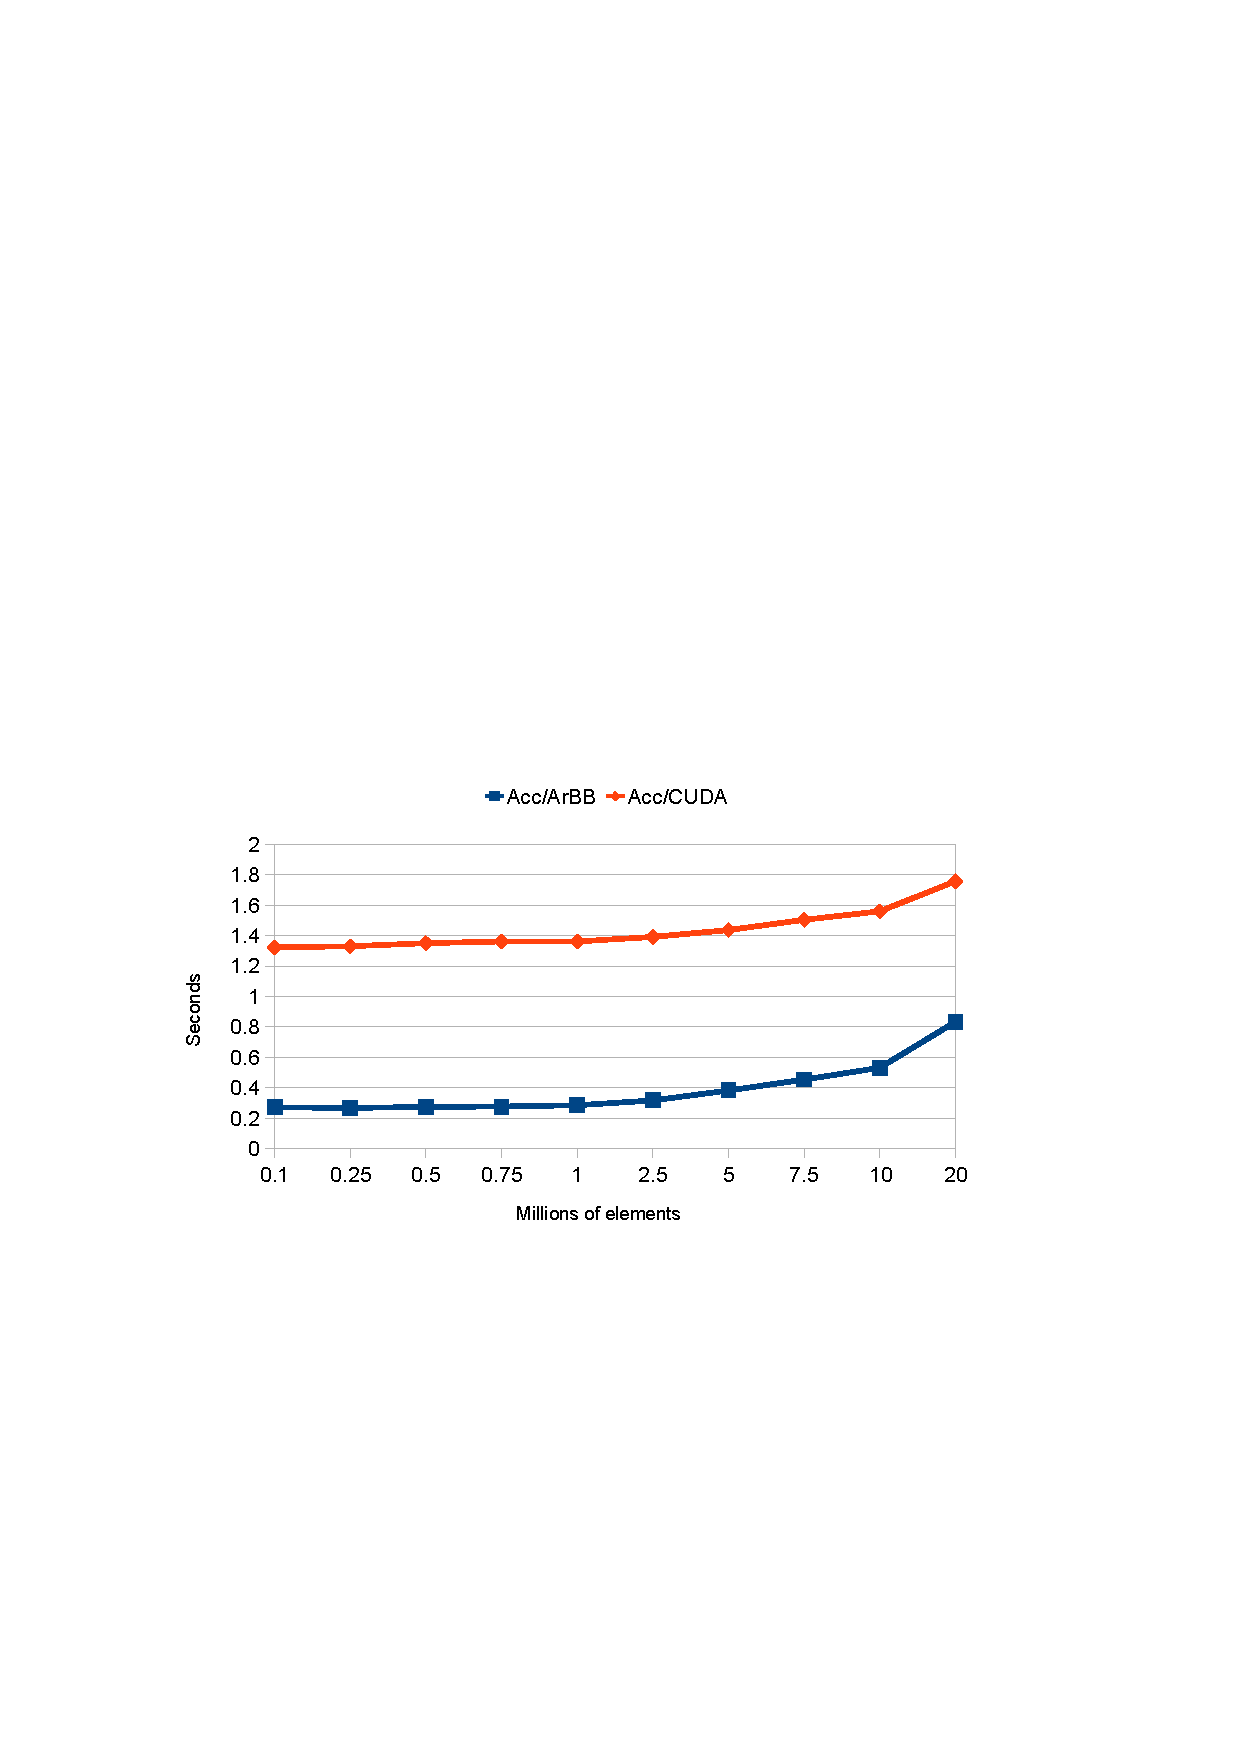
\includegraphics[width=3.5in]{./arbb/jit}    
  \end{center}
\vspace{-5mm}
  \caption{Running time experiments including JIT-time.} 
  \label{f:jit}
\end{figure}

\begin{figure}
  \begin{center}
   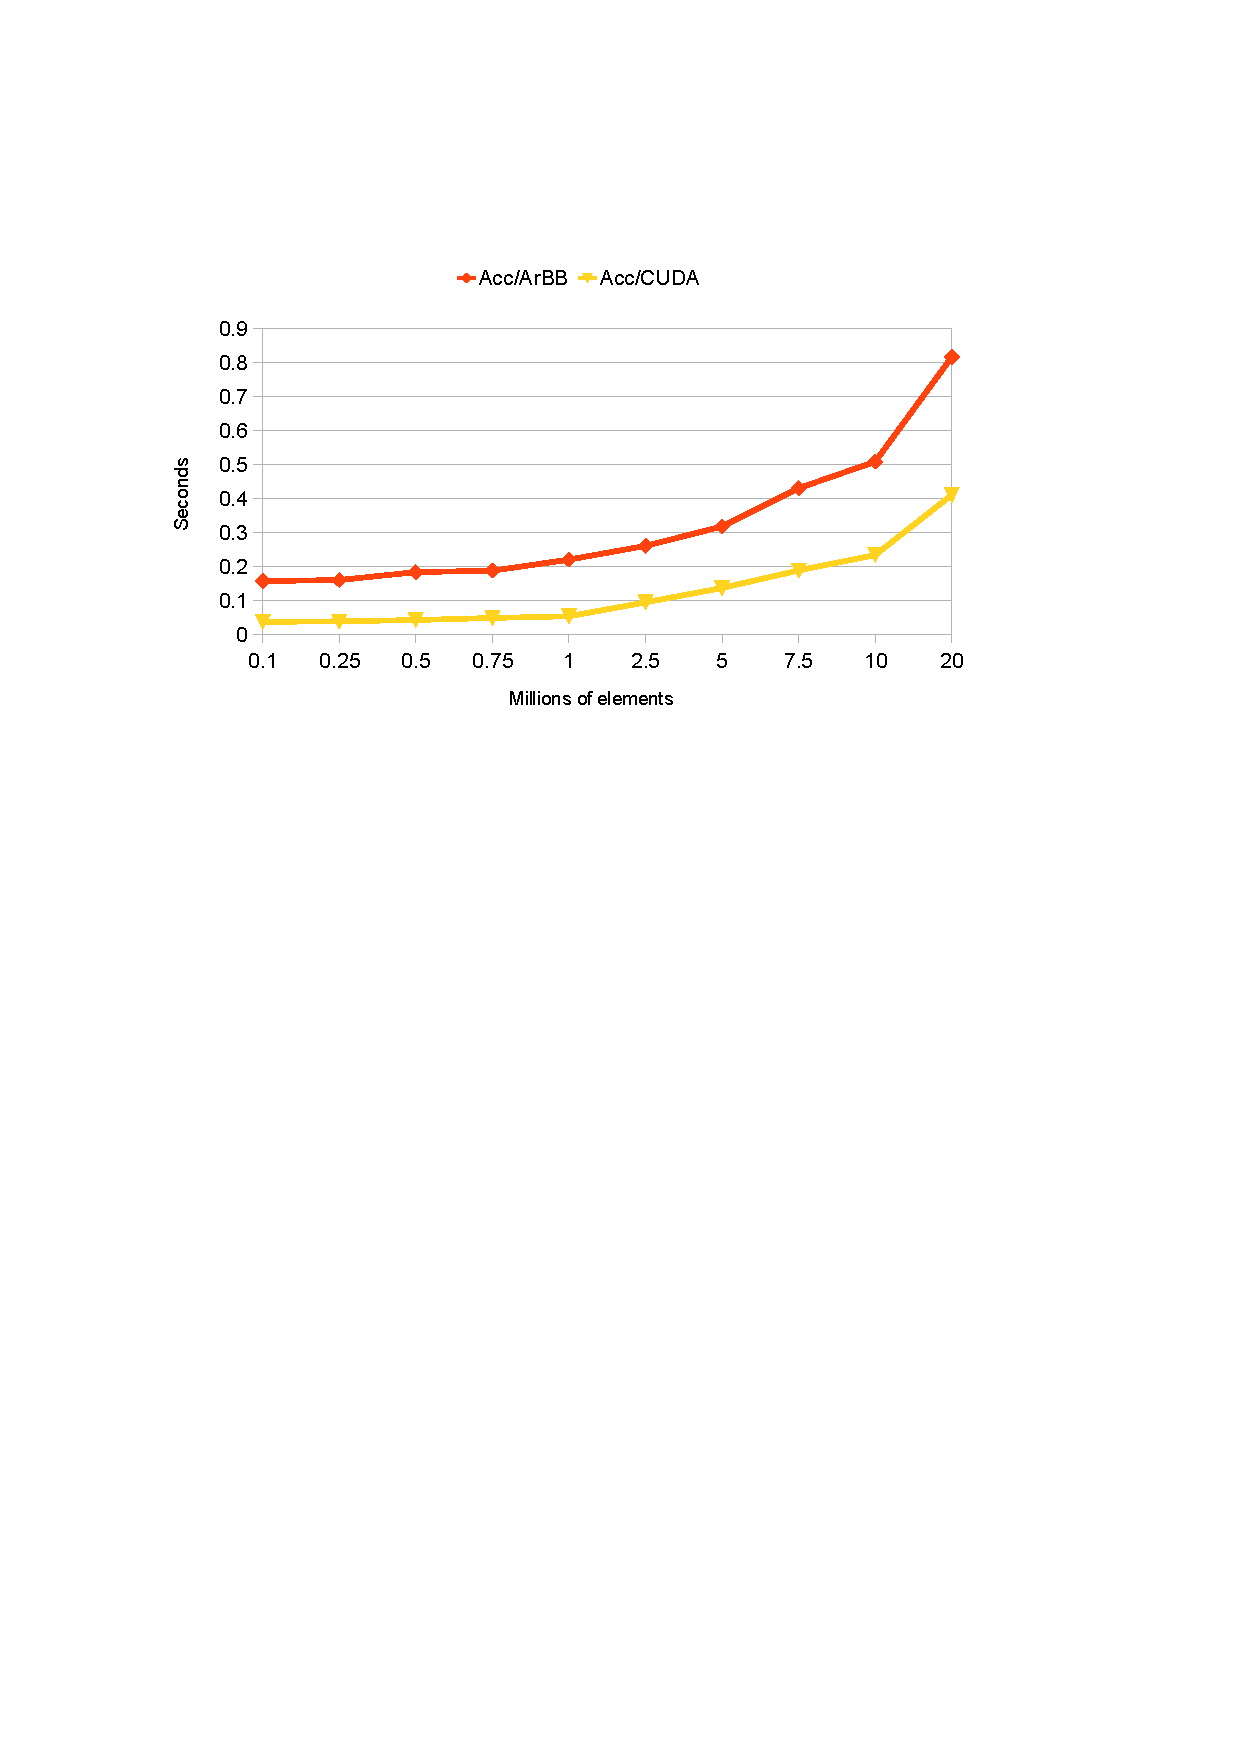
\includegraphics[width=3.5in]{./arbb/nojit}    
  \end{center}
\vspace{-5mm}
  \caption{Running time experiments JIT-time excluded.}
  \label{f:nojit}
\end{figure}


Figures~\ref{f:jit} and \ref{f:nojit} show preliminary results obtained on 
the Black-Scholes benchmark. The figures where obtained on a system with a 4-core 
Intel Core I7 975 machine with HyperThreading. The GPU used was a NVIDIA GTX480.

Figure~\ref{f:jit} shows running times obtained when JIT-time is included. 
% What this figure mainly tells us is that the JITing overhead 
JIT compilation time is much larger 
in the CUDA backend than the ArBB one.  Part of this difference 
can be attributed to the fact that 
the CUDA backend calls an external compiler (\cde{nvcc}), which takes its input in a file and runs in
a separate process.  ArBB, on the other hand, has a library interface to its  JIT-compiler. 
Figure~\ref{f:nojit} shows results obtained when pre-compiling the
CUDA functions eliminating JIT overhead.
In Accelerate, this happens automatically when the same kernel is
invoked repeatedly, because the Accelerate CUDA backed 
uses a caching scheme to avoid unnecessary JIT invocations.  (The
caching functionality has not yet been duplicated in the 
ArBB backend.)

These early results demonstrates the principle that even when a kernel
executes with higher throughput on a GPU, in a particular program it
is difficult to decide whether a computation is worth moving to a GPU,
incurring extra data-movement and possibly extra JIT compilation
\cite{wheres-the-data-paper}.  Specifically, we see that the
Accelerate Black-Scholes program from Figure~\ref{fig:blackscholes}
performs better on the CPU if it executes once (even on a large window
of data) whereas the GPU would yield better performance in a sustained
series of executions.
%
Because both CPU and GPU execution may be desirable---and the
selection may be dynamic---it is beneficial to have a single source code
that is portable across both.  
% Accelerate combined with \systemname{} makes this possible.


% ====================================================================================================
\subsection{Related Work}
% ====================================================================================================


OpenCL~\cite{opencl08} is a programming model very similar to CUDA but with the aspiration 
to offer both acceleration of computations on GPUs or to multicore CPUs. 
OpenCL JIT compiles the kernels for the particular hardware available and is
in that sense similar to ArBB.  
OpenCL programs are relatively low-level and require a large amount of
boilerplate to create and invoke.  In this sense they occupy a very
different niche than Accelerate.

Microsoft Accelerator~\cite{ACCELERATOR} is an embedded language with similar 
aspirations as ArBB, that is, to target a diverse range of architectures using the 
same source code. Accelerate can be used from the C\# language or the 
functional F\# language and targets GPUs or of CPUs and their
vector units.
% However, being part of the .Net framework implies limited accessibility 
%for platforms other than Microsoft Windows.  

\rn{What's the comparison with our stuff?}

%Most work on partitioning workloads between 
Many CPU and GPU comparisons, and some CPU/GPU workload partitioners \cite{merge}, rely on
redundant hand-written versions of all kernels
% \cite{cpu-gpu-partitioning} 
(though some systems like Qilin \cite{qilin} allow a single source code).
It is difficult in this kind of scenario
to make fair comparisons, controlling for the
amount of effort put into the respective implementations.
For example, comparing unoptimized serial CPU implementations vs. GPU
ones is not informative \cite{debunking-dubey}.
In \systemname{} controlling for effort
need happen only once---both CUDA and ArBB are
independently optimized by their respective teams of engineers---not for each benchmark.


% ====================================================================================================
% \section{Future work and Conclusions}
%\section{Future Work}
% ====================================================================================================

%\rn{need to be careful about being too repetitive...}
%The \accarbb{} backend is currently work-in-progress. The Accelerate
%functionality is not yet completely covered by the ArBB backend. Currently 
%the ArBB back-ed is operational for Accelerate programs using {\em Map}, 
%{\em ZipWith} and some simple instances of the Accelerate {\em Fold} operation.
%All of these also have the limitation that they only work for up to and 
%including 3-dimensional arrays using the ArBB backend while the Accelerate
%model allows the N-dimensional case. Allowing the N-dimensional case 
%in the ArBB backend for the supported operations range from a simple exercise 
%to more intricate problems needing some thought. For example, in the case 
%{\em Map} operations the needed transformation is simple (Accelerate Maps 
%over N-dimensional arrays is a per-element operation). One could flatten 
%the N-dimensional array to a 1-dimensional array (remembering its old shape) 
%perform the map and then transform the array back into N-dimensions. In 
%the case of {\em Fold} (reductions) the situation becomes more tricky. 
%transforming the arrays to arrays of lesser dimensionality then requires 
%a so-called segmented {\em Fold} operation. 

%The current \accarbb{} backend uses a hybrid of immediate-mode 
%and retained-mode programming styles. Moving more towards 
%retained-mode only may have performance benefits since it would give the 
%ArBB compiler larger programs to optimize. Exploring this aspect is left 
%as future work. 

% ====================================================================================================
\subsection{Discussion and Conclusions}
% ====================================================================================================

We have demonstrated that an EDSL such as Accelerate is sufficiently
platform-independent to break free of its original hardware target
(CUDA/GPU) and create efficient programs on other architectures.  This
gives us hope that \systemname{}/Accelerate programs will be
forward-portable to future parallel architectures and instruction
sets.

The EDSL approach changes the playing field for the designer
of compiler backends.  Rather than contending with full blown
languages and their complexities (e.g. pointers, aliasing,
inheritance, virtual functions, etc), compiler backends can focus on
simple value-oriented compute languages.

%% Achieving the ultimate goal of performance portability requires
%% progress on two research problems.  The first is EDSLs themselves and
%% their integration into host languages.  The second problem 

But the EDSL method solves only part of the performance-portability problem.
Simple as EDSL target languages may be, there remains a
substantial challenge in mapping them efficiently to the diversity
of parallel architectures available now and in the near future.
%especially without requiring a large amount of additional per-platform
%user annotations.
\textred{For example, the idiosyncrasies of memory bank access on
  NVIDIA GPUs must be taken into account to generate efficient
  implementations of the high-level collective operations that we have
  discussed.}

This is a compiler backend research challenge.
The {\em skeletons} method mentioned in
Section~\ref{sec:accelerate-arbb} is one approach to this problem, as
are the optimizations studied in the Copperhead \cite{copperhead} and
Obsidian \cite{OBSIDIAN-TECHREPORT} projects.
%
On the other hand, systems that rely on advanced optimizations
typically suffer to some extent from performance-predictability
problems.  Thus achieving portable, predictable performance on a wide range
of architectures---even for the simplest target languages---will
be the subject of much future work.

%{
%\small
% \bibliographystyle{plainnat}
%\bibliographystyle{IEEEtran}
%\bibliography{IEEEabrv,haskell_arbb}
%}


%\end{document}


